\documentclass{beamer}
\usepackage{isabelle,isabellesym}


\isabellestylett

\addtobeamertemplate{navigation symbols}{}{%
    \usebeamerfont{footline}%
    \usebeamercolor[fg]{footline}%
    \hspace{1em}%
    \insertframenumber/\inserttotalframenumber
}


\title{Isabelle/HOL on Fork Prevention\\ in the Coming Ethereum Protocol}
\author{Yoichi Hirai\\ {\small Ethereum Foundation}}
\date{Berlin, 30 Aug. 2017}

\begin{document}

\begin{frame}
\titlepage
\end{frame}

\begin{frame}{What is Ethereum}

Ethereum is one instance of a virtual machine, which is
\begin{itemize}
\item as powerful as a 20-year-old smart phone
\item replicated globally
\item with no central parties
\item running for 2 years by now
\end{itemize}

\vfill

\structure{How does Ethereum synchronize execution traces?} \\
Asynchronous communication cannot establish new common knowledge [Chandy \& Misra, 1986].
\end{frame}

\begin{frame}{A Blockchain}
is just a data strucuture.  It is a tree, not a chain.

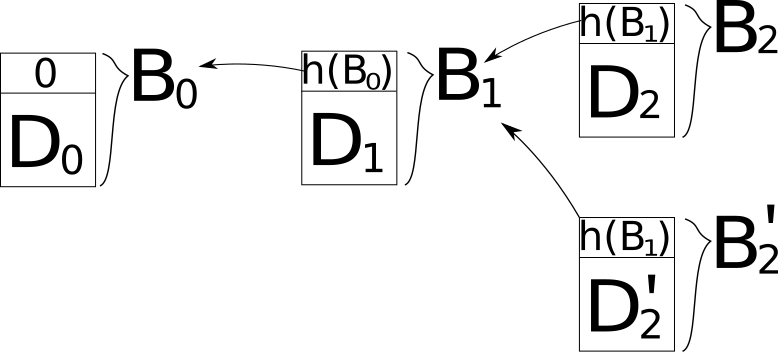
\includegraphics[width=\textwidth]{blockchains.png}

A small number $h(B_n)$ identifies a sequence $B_0, \ldots B_n$ and \\
moreover, in Ethereum, the execution trace of a virtual machine.

\end{frame}


\begin{frame}{Proof of Work}

\begin{itemize}
\item a block's content $D$ needs to contain a nicely chosen nonce\\ so that the hash $h(D)$ of the block is small enough
\item when you find such a nonce, the protocol gives reward in your account (in the state after the block)
\item account?
\end{itemize}

Finding a good nonce is called \structure{mining}.
\vfill
I belive nobody has found a better way than brute-forcing.
\vfill
``Ethereum miners are renting Boeing 747s to ship graphics cards and AMD shares are soaring'' ({\tiny\url{https://qz.com/1039809}})\\
(sounds a bit like Moai's).
\end{frame}

\begin{frame}{Proof of Work}

\structure{If you succeed creating a block}
\begin{enumerate}
\item the block reward is only spendable in chains that include your block
\item you should send around the block, maybe
\end{enumerate}

\structure{If you see a block being sent around}
\begin{enumerate}
\item if that's the best block you've seen, you should try to mine on the block \\
      (assumption: absense of complicated motives, other nodes' straightforward behavior)
\item you should broadcast the block you are mining on, maybe
\end{enumerate}

\vfill

\structure{Does it work?}  Yes, see Bitcoin.

\structure{Why?}  I don't know, honestly.
\end{frame}

\begin{frame}{Evaluating Proof of Work}

No good properties distributed-computation-wise.

(A good leader-election protocol can tolerate less than 1/3 Byzantine nodes.)

\structure{One Byzantine node can}
\begin{itemize}
\item be lucky enough to guess the secret keys of everyone.
\end{itemize}

\structure{One (economically) irrational node can}
\begin{itemize}
\item buy lots of machines to mine quicker than anybody,\\ rewriting the history from any point in the past.
\end{itemize}

\structure{Why this ``algorithm''?} \underline{number of nodes} is not reliable.

Instead, Proof-of-Work uses electricity consumption (or luck).

Instead, Proof-of-Stake uses in-protocol deposit.

These designs require numbers that carry values associated to public keys.

\end{frame}


\begin{frame}{Proof-of-Stake}

\begin{itemize}
\item Replacing GPU and electricity with deposits of in-protocol tokens.
\item A difference: in-protocol tokens duplicate as forks happen.
\item Solution: provably dishonest behavior is punished on all forks.
\end{itemize}

\alert{Slash those who's active on multiple chains!}\\ is too intimidating.
\end{frame}


\begin{frame}{I Received a Challenge: Original Text}

  \structure{Message types}

  \begin{itemize}
  \item commit(HASH, view)
  \item prepare(HASH, view, view\_source),\\ -1 $\le$ view\_source $<$ view
  \end{itemize}

  \structure{Slashing conditions}

  \begin{enumerate}
    \item commit(H, v) REQUIRES 2/3 prepare(H, v, vs) for some consistent vs
    \item prepare(H, v, vs) REQUIRES 2/3 prepare(H\_anc, vs, vs') for some consistent vs', where H\_anc is a (v-vs)-degree ancestor of H, UNLESS vs = -1
    \item commit(H, v) + prepare(H, w, u) ILLEGAL if u $<$ v $<$ w
    \item prepare(X1, v, vs1) + prepare(X2, v, vs2) ILLEGAL\\ unless X1 = X2 and vs1 = vs2
  \end{enumerate}

\end{frame}

\begin{frame}{Challenge Continued}

  \structure{Accountable safety argument}\\ (proof path - assume two incompatible values got committed, show 1/3+ SLASHED)

  \structure{Case 1}

\quad 2/3 commit(X, v) \& 2/3 commit(Y, v)

$\rightarrow$ 2/3 prepare(X, v, vs) \& 2/3 prepare(Y, v, vs')  (\structure{1.})

$\rightarrow$ 1/3 SLASHED (\structure{4.})

\structure{Case 2}

\quad 2/3 commit(Y, v2) \& 2/3 commit(X, v1),\\ Y is NOT a (v2-v1)-degree descendant of X, define Y[i] to be the ancestor of Y in view i

$\rightarrow$ 2/3 prepare(Y[v2], v2, vs), vs $<$ v2 (\structure{1.})

$\rightarrow$ 2/3 prepare(Y[vs], vs, vs') (\structure{2.})

$\rightarrow$ ...

[continue induction until vs' $<$ v1]

(Two base cases follow.)

\end{frame}

\begin{frame}{Alloy modelling}
Being unsure what the definitions meant, I turned to Alloy.

Alloy \url{http://alloy.mit.edu/alloy/} is a prototyping-tool.
\vfill
You can type in definitions, assumptiions and a conjecture \\
in relational algebra (a bit more expressible than FOL).
\vfill
Alloy tries to find a counterexample.  No guarantees of false-negatives.
\end{frame}

\begin{frame}[fragile]{Alloy example}

\begin{verbatim}
sig View { v_prev: lone View }

sig Hash { h_prev: lone Hash }

fact { no x : Hash | x in x.(^h_prev) }

sig Prepare { hash : Hash,
              view : View,
              view_src : View }

fact{ all p : Prepare | p.view_src in (p.view.(^v_prev))}

pred some_prepare { some Prepare }

run some_prepare for 3
\end{verbatim}

\end{frame}

\begin{frame}
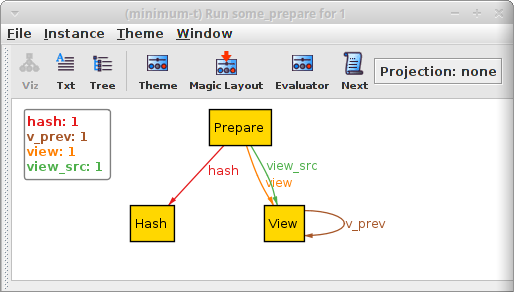
\includegraphics[width=\textwidth]{circle.png}
\end{frame}

\begin{frame}[fragile]{Somehow I can code the Slashing Conditions}

Text: commit(H, v) REQUIRES 2/3 prepare(H, v, vs) for some consistent vs

\begin{verbatim}
// Slashing condition [i]
pred slashed1 (s : Node) {
   some c : Commit |
      s in c.c_sender &&
      (#{n : Node | some p : Prepare |
            p.p_sender = n
         && p.p_hash = c.c_hash})

     . mul[ 3]
     < mul[ #{n : Node}, 2 ]
}
\end{verbatim}

etc.
\end{frame}

\begin{frame}[fragile]{I can also define a fork with 2/3 non-slashed nodes}

\begin{verbatim}
pred incompatible_commits {
   some Node &&
   some h0, h1 : Hash |
    (not h0 in h1.(*h_prev)) &&
    (not h1 in h0.(*h_prev)) &&
    (#{n0 : Node |
         some c0 : Commit |
         c0.c_sender = n0 && c0.c_hash = h0}
    ).mul[3] >= (#Node).mul[2] &&
    (#{n1 : Node |
         some c1 : Commit |
         c1.c_sender = n1 && c1.c_hash = h1}
    ).mul[3] >= (#Node).mul[2] &&
    (#SlashedNode).mul[3] < (#Node)
}
\end{verbatim}

Now Alloy, go find incompatible commits.
\end{frame}

\begin{frame}{Fork?}
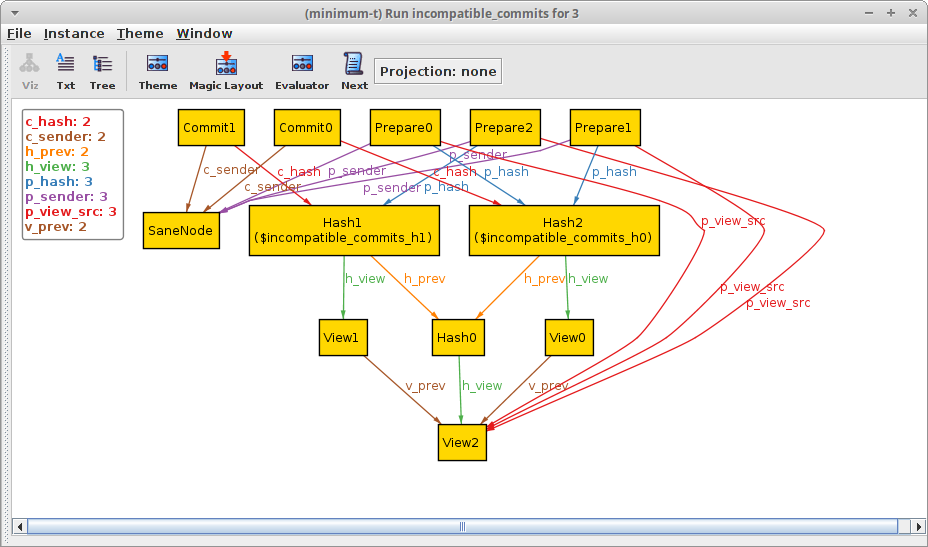
\includegraphics[width=\textwidth]{fork.png}

\only<2->{Mistake: I forgot to specify Views have a total order.}
\end{frame}

\begin{frame}{Another Fork?}
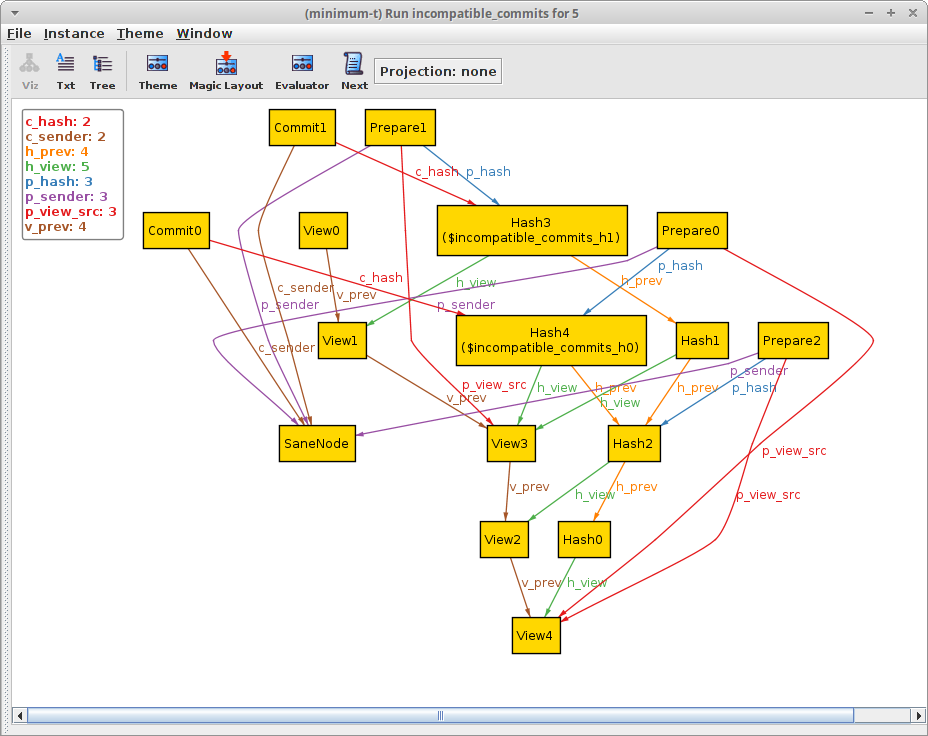
\includegraphics[width=\textwidth]{fork2.png}
\end{frame}

\begin{frame}[fragile]{Another Fork?  Mistake}

``prepare(H, v, vs) REQUIRES 2/3 prepare(H\_anc, vs, vs') for some consistent vs', \alert{where H\_anc is a (v-vs)-degree ancestor of H}, UNLESS vs = -1''

\begin{verbatim}
fact {
   all p : Prepare |
      (p.p_sender in SaneNode && some p.p_view_src.v_prev) implies
      some h_anc : Hash | some v_src : View |
      h_anc in p.p_hash.(^h_prev) &&
+     h_anc.h_view = p.p_view_src &&
       (#{n : Node | some p' : Prepare | p'.p_sender = n
              && p'.p_hash = h_anc && p'.p_view_src = v_src })
        . mul[ 3]  >= (#{n : Node}).mul[ 2 ]
}
\end{verbatim}
\end{frame}

\begin{frame}{Prepare2 does not justify Prepare1}
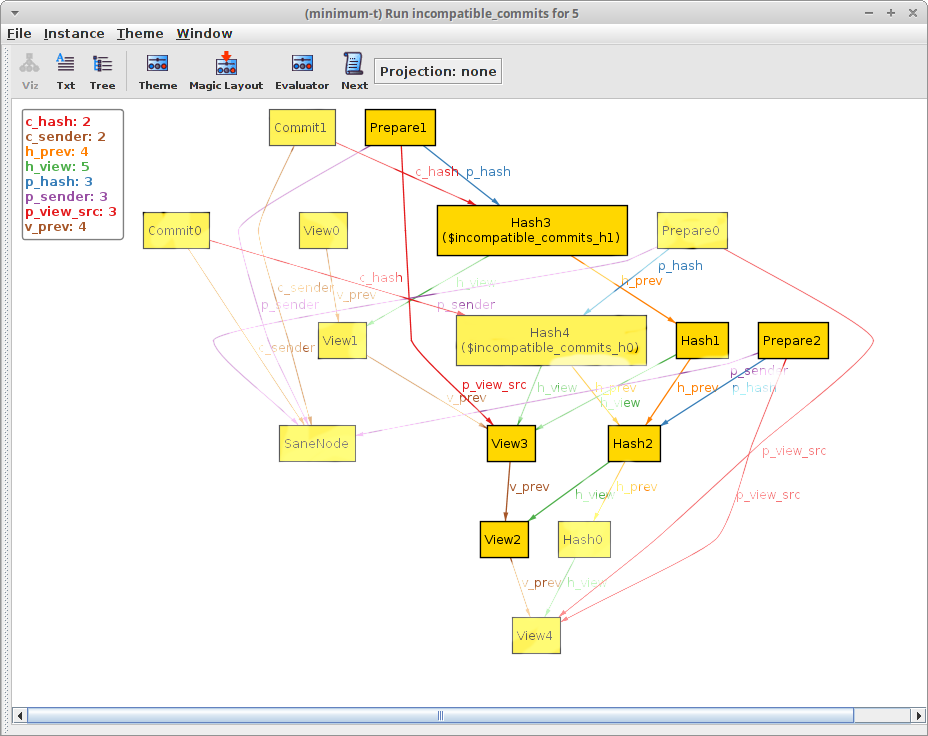
\includegraphics[width=\textwidth]{fork3.png}
\end{frame}

\begin{frame}{Isabelle/HOL}

When I was confident I turned to Isabelle/HOL.

\vfill

\alert{Turned out followable in Isabelle/HOL (1,800 lines).}
\end{frame}

\renewcommand\isacharbar{$\mid$}

\begin{frame}{Messages and Validators}

\isacommand{datatype}\isamarkupfalse%
\ hash\ {\isacharequal}\ Hash\ int%

\isacommand{type{\isacharunderscore}synonym}\isamarkupfalse%
\ view\ {\isacharequal}\ int%

\isacommand{datatype}\isamarkupfalse%
\ message\ {\isacharequal}\isanewline
\ \ Commit\ {\isachardoublequoteopen}hash\ {\isacharasterisk}\ view{\isachardoublequoteclose}\isanewline
{\isacharbar}\ Prepare\ {\isachardoublequoteopen}hash\ {\isacharasterisk}\ view\ {\isacharasterisk}\ view{\isachardoublequoteclose}%

\isacommand{datatype}\isamarkupfalse%
\ validator\ {\isacharequal}\ Validator\ int%

\isacommand{type{\isacharunderscore}synonym}\isamarkupfalse%
\ signed{\isacharunderscore}message\ {\isacharequal}\ {\isachardoublequoteopen}validator\ {\isacharasterisk}\ message{\isachardoublequoteclose}%
\end{frame}

\begin{frame}{Situation}

\isacommand{record}\isamarkupfalse%
\ situation\ {\isacharequal}\isanewline
\ \ Validators\ {\isacharcolon}{\isacharcolon}\ {\isachardoublequoteopen}validator\ set{\isachardoublequoteclose}\isanewline
\ \ Messages\ {\isacharcolon}{\isacharcolon}\ {\isachardoublequoteopen}signed{\isacharunderscore}message\ set{\isachardoublequoteclose}\isanewline
\ \ PrevHash\ {\isacharcolon}{\isacharcolon}\ {\isachardoublequoteopen}hash\ {\isasymRightarrow}\ hash\ option{\isachardoublequoteclose}%

\end{frame}


\renewcommand\isacharunderscore{\_}


\begin{frame}{Ancestors}

\isacommand{fun}\isamarkupfalse%
\ nth{\isacharunderscore}ancestor\ {\isacharcolon}{\isacharcolon}\ {\isachardoublequoteopen}situation\ {\isasymRightarrow}\ nat\ {\isasymRightarrow}\ hash\ {\isasymRightarrow}\ hash\ option{\isachardoublequoteclose}\isanewline
\isakeyword{where}\isanewline
\ \ {\isachardoublequoteopen}nth{\isacharunderscore}ancestor\ {\isacharunderscore}\ {\isadigit{0}}\ h\ {\isacharequal}\ Some\ h{\isachardoublequoteclose}\isanewline
{\isacharbar}\ {\isachardoublequoteopen}nth{\isacharunderscore}ancestor\ s\ {\isacharparenleft}Suc\ n{\isacharparenright}\ h\ {\isacharequal}\isanewline
\ \ \ {\isacharparenleft}case\ PrevHash\ s\ h\ of\isanewline
\ \ \ \ \ \ None\ {\isasymRightarrow}\ None\isanewline
\ \ \ \ {\isacharbar}\ Some\ h{\isacharprime}\ {\isasymRightarrow}\ nth{\isacharunderscore}ancestor\ s\ n\ h{\isacharprime}{\isacharparenright}{\isachardoublequoteclose}%

\end{frame}

\begin{frame}
\isacommand{definition}\isamarkupfalse%
\ is{\isacharunderscore}descendant{\isacharunderscore}or{\isacharunderscore}self\ {\isacharcolon}{\isacharcolon}\ {\isachardoublequoteopen}situation\ {\isasymRightarrow}\ hash\ {\isasymRightarrow}\ hash\ {\isasymRightarrow}\ bool{\isachardoublequoteclose}\isanewline
\isakeyword{where}\isanewline
           {\isachardoublequoteopen}is{\isacharunderscore}descendant{\isacharunderscore}or{\isacharunderscore}self\ s\ x\ y\ {\isacharequal}\ {\isacharparenleft}{\isasymexists}\ n{\isachardot}\ nth{\isacharunderscore}ancestor\ s\ n\ x\ {\isacharequal}\ Some\ y{\isacharparenright}{\isachardoublequoteclose}%

           \vfill
\isacommand{definition}\isamarkupfalse%
\ not{\isacharunderscore}on{\isacharunderscore}same{\isacharunderscore}chain\ {\isacharcolon}{\isacharcolon}\ {\isachardoublequoteopen}situation\ {\isasymRightarrow}\ hash\ {\isasymRightarrow}\ hash\ {\isasymRightarrow}\ bool{\isachardoublequoteclose}\isanewline
\isakeyword{where}\isanewline
{\isachardoublequoteopen}not{\isacharunderscore}on{\isacharunderscore}same{\isacharunderscore}chain\ s\ x\ y\ {\isacharequal}\ {\isacharparenleft}{\isacharparenleft}{\isasymnot}\ is{\isacharunderscore}descendant{\isacharunderscore}or{\isacharunderscore}self\ s\ x\ y{\isacharparenright}\ {\isasymand}\ {\isacharparenleft}{\isasymnot}\ is{\isacharunderscore}descendant{\isacharunderscore}or{\isacharunderscore}self\ s\ y\ x{\isacharparenright}{\isacharparenright}{\isachardoublequoteclose}%
\end{frame}

\renewcommand{\isacharbraceleft}{\{}
\renewcommand{\isacharbraceright}{\}}

\begin{frame}
\isacommand{definition}\isamarkupfalse%
\ two{\isacharunderscore}thirds\ {\isacharcolon}{\isacharcolon}\ {\isachardoublequoteopen}situation\ {\isasymRightarrow}\ {\isacharparenleft}validator\ {\isasymRightarrow}\ bool{\isacharparenright}\ {\isasymRightarrow}\ bool{\isachardoublequoteclose}\isanewline
\isakeyword{where}\isanewline
{\isachardoublequoteopen}two{\isacharunderscore}thirds\ s\ f\ {\isacharequal}\isanewline
\ \ \ {\isacharparenleft}{\isadigit{2}}\ {\isacharasterisk}\ card\ {\isacharparenleft}Validators\ s{\isacharparenright}\ {\isasymle}\\\ \ \ \  {\isadigit{3}}\ {\isacharasterisk}\ card\ {\isacharparenleft}{\isacharbraceleft}n{\isachardot}\ n\ {\isasymin}\ Validators\ s\ {\isasymand}\ f\ n{\isacharbraceright}{\isacharparenright}{\isacharparenright}{\isachardoublequoteclose}%
\end{frame}

\begin{frame}
\isacommand{definition}\isamarkupfalse%
\ prepared\ {\isacharcolon}{\isacharcolon}\ {\isachardoublequoteopen}situation\ {\isasymRightarrow}\ hash\ {\isasymRightarrow}\ view\ {\isasymRightarrow}\ view\ {\isasymRightarrow}\ bool{\isachardoublequoteclose}\isanewline
\isakeyword{where}\isanewline
{\isachardoublequoteopen}prepared\ s\ h\ v\ vs\ {\isacharequal}\isanewline
\ \ \ {\isacharparenleft}two{\isacharunderscore}thirds{\isacharunderscore}sent{\isacharunderscore}message\ s\ {\isacharparenleft}Prepare\ {\isacharparenleft}h{\isacharcomma}\ v{\isacharcomma}\ vs{\isacharparenright}{\isacharparenright}{\isacharparenright}{\isachardoublequoteclose}%
\vfill
\isacommand{definition}\isamarkupfalse%
\ committed\ {\isacharcolon}{\isacharcolon}\ {\isachardoublequoteopen}situation\ {\isasymRightarrow}\ hash\ {\isasymRightarrow}\ bool{\isachardoublequoteclose}\isanewline
\isakeyword{where}\isanewline
           {\isachardoublequoteopen}committed\ s\ h\ {\isacharequal}\\
           \ \ \ \ {\isacharparenleft}{\isasymexists}\ v{\isachardot}\ two{\isacharunderscore}thirds{\isacharunderscore}sent{\isacharunderscore}message\ s\ {\isacharparenleft}Commit\ {\isacharparenleft}h{\isacharcomma}\ v{\isacharparenright}{\isacharparenright}{\isacharparenright}{\isachardoublequoteclose}%
\isamarkupsection{The Slashing Conditions (not skippable)%
}
\isamarkuptrue%
%
\end{frame}

\begin{frame}
\begin{isamarkuptext}%
[i] A validator is slashed when it has sent a commit message of a hash
      that is not prepared yet.%
\end{isamarkuptext}\isamarkuptrue%
\isacommand{definition}\isamarkupfalse%
\ slashed{\isacharunderscore}one\ {\isacharcolon}{\isacharcolon}\ {\isachardoublequoteopen}situation\ {\isasymRightarrow}\ validator\ {\isasymRightarrow}\ bool{\isachardoublequoteclose}\isanewline
\isakeyword{where}\isanewline
{\isachardoublequoteopen}slashed{\isacharunderscore}one\ s\ n\ {\isacharequal}\isanewline
\ {\isacharparenleft}n\ {\isasymin}\ Validators\ s\ {\isasymand}\isanewline
\ \ \ \ {\isacharparenleft}{\isasymexists}\ h\ v{\isachardot}\isanewline
\ \ \ \ \ \ {\isacharparenleft}{\isacharparenleft}n{\isacharcomma}\ Commit\ {\isacharparenleft}h{\isacharcomma}\ v{\isacharparenright}{\isacharparenright}\ {\isasymin}\ Messages\ s\ {\isasymand}\isanewline
\ \ \ \ {\isacharparenleft}{\isasymnot}\ {\isacharparenleft}{\isasymexists}\ vs{\isachardot}\ {\isacharminus}{\isadigit{1}}\ {\isasymle}\ vs\ {\isasymand}\ vs\ {\isacharless}\ v\ {\isasymand}\ prepared\ s\ h\ v\ vs{\isacharparenright}\ {\isacharparenright}{\isacharparenright}{\isacharparenright}{\isacharparenright}{\isachardoublequoteclose}%
\end{frame}

\begin{frame}
\begin{isamarkuptext}%
[ii] A validator is slashed when it has sent a prepare message whose
      view src is not -1 but has no supporting preparation in the view src.%
\end{isamarkuptext}\isamarkuptrue%
\isacommand{definition}\isamarkupfalse%
\ slashed{\isacharunderscore}two\ {\isacharcolon}{\isacharcolon}\ {\isachardoublequoteopen}situation\ {\isasymRightarrow}\ validator\ {\isasymRightarrow}\ bool{\isachardoublequoteclose}\isanewline
\isakeyword{where}\isanewline
{\isachardoublequoteopen}slashed{\isacharunderscore}two\ s\ n\ {\isacharequal}\isanewline
\ \ {\isacharparenleft}n\ {\isasymin}\ Validators\ s\ {\isasymand}\isanewline
\ \ \ \ \ {\isacharparenleft}{\isasymexists}\ h\ v\ vs{\isachardot}\isanewline
\ \ \ \ \ \ \ {\isacharparenleft}{\isacharparenleft}n{\isacharcomma}\ Prepare\ {\isacharparenleft}h{\isacharcomma}\ v{\isacharcomma}\ vs{\isacharparenright}{\isacharparenright}\ {\isasymin}\ Messages\ s\ {\isasymand}\isanewline
\ \ \ \ \ \ \ vs\ {\isasymnoteq}\ {\isacharminus}{\isadigit{1}}\ {\isasymand}\isanewline
\ \ \ \ \ \ \ {\isacharparenleft}{\isasymnot}\ {\isacharparenleft}{\isasymexists}\ h{\isacharunderscore}anc\ vs{\isacharprime}{\isachardot}\isanewline
\ \ \ \ \ \ \ \ \ \ \ {\isacharminus}{\isadigit{1}}\ {\isasymle}\ vs{\isacharprime}\ {\isasymand}\ vs{\isacharprime}\ {\isacharless}\ vs\ {\isasymand}\isanewline
\ \ \ \ \ \ \ \ \ \ \ Some\ h{\isacharunderscore}anc\ {\isacharequal}\ nth{\isacharunderscore}ancestor\ s\ {\isacharparenleft}nat\ {\isacharparenleft}v\ {\isacharminus}\ vs{\isacharparenright}{\isacharparenright}\ h\ {\isasymand}\isanewline
\ \ \ \ \ \ \ \ \ \ \ prepared\ s\ h{\isacharunderscore}anc\ vs\ vs{\isacharprime}{\isacharparenright}{\isacharparenright}{\isacharparenright}{\isacharparenright}{\isacharparenright}{\isachardoublequoteclose}%
\end{frame}

\begin{frame}
\begin{isamarkuptext}%
[iii] A validator is slashed when it has sent a commit message and a prepare message
     containing view numbers in a specific constellation.%
\end{isamarkuptext}\isamarkuptrue%
\isacommand{definition}\isamarkupfalse%
\ slashed{\isacharunderscore}three\ {\isacharcolon}{\isacharcolon}\ {\isachardoublequoteopen}situation\ {\isasymRightarrow}\ validator\ {\isasymRightarrow}\ bool{\isachardoublequoteclose}\isanewline
\isakeyword{where}\isanewline
{\isachardoublequoteopen}slashed{\isacharunderscore}three\ s\ n\ {\isacharequal}\isanewline
\ \ {\isacharparenleft}n\ {\isasymin}\ Validators\ s\ {\isasymand}\isanewline
\ \ \ \ {\isacharparenleft}{\isasymexists}\ x\ y\ v\ w\ u{\isachardot}\isanewline
\ \ \ \ \ \ {\isacharparenleft}n{\isacharcomma}\ Commit\ {\isacharparenleft}x{\isacharcomma}\ v{\isacharparenright}{\isacharparenright}\ {\isasymin}\ Messages\ s\ {\isasymand}\isanewline
\ \ \ \ \ \ {\isacharparenleft}n{\isacharcomma}\ Prepare\ {\isacharparenleft}y{\isacharcomma}\ w{\isacharcomma}\ u{\isacharparenright}{\isacharparenright}\ {\isasymin}\ Messages\ s\ {\isasymand}\isanewline
\ \ \ \ \ \ u\ {\isacharless}\ v\ {\isasymand}\ v\ {\isacharless}\ w{\isacharparenright}{\isacharparenright}{\isachardoublequoteclose}%
\end{frame}

\begin{frame}
\begin{isamarkuptext}%
[iv] A validator is slashed when it has signed two different Prepare messages at the same view.%
\end{isamarkuptext}\isamarkuptrue%
\isacommand{definition}\isamarkupfalse%
\ slashed{\isacharunderscore}four\ {\isacharcolon}{\isacharcolon}\ {\isachardoublequoteopen}situation\ {\isasymRightarrow}\ validator\ {\isasymRightarrow}\ bool{\isachardoublequoteclose}\isanewline
\isakeyword{where}\isanewline
{\isachardoublequoteopen}slashed{\isacharunderscore}four\ s\ n\ {\isacharequal}\isanewline
\ \ {\isacharparenleft}n\ {\isasymin}\ Validators\ s\ {\isasymand}\isanewline
\ \ \ \ {\isacharparenleft}{\isasymexists}\ x{\isadigit{1}}\ x{\isadigit{2}}\ v\ vs{\isadigit{1}}\ vs{\isadigit{2}}{\isachardot}\isanewline
\ \ \ \ \ \ {\isacharparenleft}n{\isacharcomma}\ Prepare\ {\isacharparenleft}x{\isadigit{1}}{\isacharcomma}\ v{\isacharcomma}\ vs{\isadigit{1}}{\isacharparenright}{\isacharparenright}\ {\isasymin}\ Messages\ s\ {\isasymand}\isanewline
\ \ \ \ \ \ {\isacharparenleft}n{\isacharcomma}\ Prepare\ {\isacharparenleft}x{\isadigit{2}}{\isacharcomma}\ v{\isacharcomma}\ vs{\isadigit{2}}{\isacharparenright}{\isacharparenright}\ {\isasymin}\ Messages\ s\ {\isasymand}\isanewline
\ \ \ \ \ \ {\isacharparenleft}x{\isadigit{1}}\ {\isasymnoteq}\ x{\isadigit{2}}\ {\isasymor}\ vs{\isadigit{1}}\ {\isasymnoteq}\ vs{\isadigit{2}}{\isacharparenright}{\isacharparenright}{\isacharparenright}{\isachardoublequoteclose}%
\end{frame}

\begin{frame}
\begin{isamarkuptext}%
A validator is slashed when at least one of the above conditions [i]--[iv] hold.%
\end{isamarkuptext}\isamarkuptrue%
\isacommand{definition}\isamarkupfalse%
\ slashed\ {\isacharcolon}{\isacharcolon}\ {\isachardoublequoteopen}situation\ {\isasymRightarrow}\ validator\ {\isasymRightarrow}\ bool{\isachardoublequoteclose}\isanewline
\isakeyword{where}\isanewline
{\isachardoublequoteopen}slashed\ s\ n\ {\isacharequal}\ {\isacharparenleft}slashed{\isacharunderscore}one\ s\ n\ {\isasymor}\isanewline
\ \ \ \ \ \ \ \ \ \ \ \ \ \ \ \ slashed{\isacharunderscore}two\ s\ n\ {\isasymor}\isanewline
\ \ \ \ \ \ \ \ \ \ \ \ \ \ \ \ slashed{\isacharunderscore}three\ s\ n\ {\isasymor}\isanewline
\ \ \ \ \ \ \ \ \ \ \ \ \ \ \ \ slashed{\isacharunderscore}four\ s\ n{\isacharparenright}{\isachardoublequoteclose}\isanewline
\isanewline
\isacommand{definition}\isamarkupfalse%
\ one{\isacharunderscore}third{\isacharunderscore}slashed\ {\isacharcolon}{\isacharcolon}\ {\isachardoublequoteopen}situation\ {\isasymRightarrow}\ bool{\isachardoublequoteclose}\isanewline
\isakeyword{where}\isanewline
{\isachardoublequoteopen}one{\isacharunderscore}third{\isacharunderscore}slashed\ s\ {\isacharequal}\ one{\isacharunderscore}third\ s\ {\isacharparenleft}slashed\ s{\isacharparenright}{\isachardoublequoteclose}%
\end{frame}

\begin{frame}{Conclusion}
\begin{isamarkuptext}%
The statement of accountable safety is simple.  If a situation has a finite number of validators (but not zero),
if two hashes x and y are committed in the situation, but if the two hashes are not on the same chain,
at least one-third of the validators are slashed in the situation.%
\end{isamarkuptext}\isamarkuptrue%
\isacommand{lemma}\isamarkupfalse%
\ accountable{\isacharunderscore}safety\ {\isacharcolon}\isanewline
\ \ {\isachardoublequoteopen}situation{\isacharunderscore}has{\isacharunderscore}finitely{\isacharunderscore}many{\isacharunderscore}validators\ s\ {\isasymLongrightarrow}\isanewline
\ \ \ committed\ s\ x\ {\isasymLongrightarrow}\ committed\ s\ y\ {\isasymLongrightarrow}\isanewline
\ \ \ not{\isacharunderscore}on{\isacharunderscore}same{\isacharunderscore}chain\ s\ x\ y\ {\isasymLongrightarrow}\ one{\isacharunderscore}third{\isacharunderscore}slashed\ s{\isachardoublequoteclose}\isanewline
\end{frame}

\begin{frame}{After that}
  \begin{itemize}
  \item the result was expanded to allow the validator set change
  \item The ``Casper contract'' is not verified according to these slashing conditions.
  \end{itemize}
\end{frame}

\begin{frame}{Other formal verification projects}
\begin{itemize}
\item eth-isabelle: an executable specification of Ethereum Virtual Machine in Lem: available for Isabelle/HOL too.
\item a compiler on top of eth-isabelle by @mrsmkl
\item some ongoing work on EVM1.5
\item KEVM by Grigore Rosu and his team
\end{itemize}
\end{frame}

\end{document}
